\documentclass[11pt,a4paper]{article}

% ─── Packages ────────────────────────────────────────────────────────
\usepackage[utf8]{inputenc}
\usepackage[T1]{fontenc}
\usepackage[margin=2.2cm]{geometry}
\usepackage{amsmath,amssymb,amsthm,mathtools}
\usepackage{physics}           % \tr, \norm, etc.
\usepackage{bm}
\usepackage{graphicx}
\usepackage{xcolor}
\usepackage{hyperref}
\usepackage{cleveref}
\usepackage{enumitem}
\usepackage{booktabs}
\usepackage{caption}
\usepackage{subcaption}
\usepackage{float}
%\usepackage{microtype} % not available in this TeX installation
\usepackage{tcolorbox}
\tcbuselibrary{theorems,skins}

% ─── Theorem environments ────────────────────────────────────────────
\newtheorem{theorem}{Theorem}[section]
\newtheorem{proposition}[theorem]{Proposition}
\newtheorem{lemma}[theorem]{Lemma}
\newtheorem{corollary}[theorem]{Corollary}
\newtheorem{definition}[theorem]{Definition}
\newtheorem{remark}[theorem]{Remark}
\newtheorem{example}[theorem]{Example}
\newtheorem{observation}[theorem]{Observation}

% ─── Notation shortcuts ─────────────────────────────────────────────
\newcommand{\R}{\mathbb{R}}
\newcommand{\E}{\mathbb{E}}
\newcommand{\Var}{\operatorname{Var}}
\newcommand{\Cov}{\operatorname{Cov}}
\newcommand{\diag}{\operatorname{diag}}
\newcommand{\Dt}{\Delta_t}
\newcommand{\sigeta}{\sigma_\eta^2}
\newcommand{\sigzero}{\sigma_0^2}
\newcommand{\siginf}{\sigma_\infty^2}

% ─── Key result box ─────────────────────────────────────────────────
\newtcolorbox{keyresult}[1][]{%
  colback=blue!5!white, colframe=blue!60!black,
  fonttitle=\bfseries, title={#1}, sharp corners, boxrule=0.6pt}

% ─── Title ───────────────────────────────────────────────────────────
\title{\bfseries The Structure of $\Sigma_t$ and $\Sigma_t^{-1}$\\[4pt]
in the AR(1) Diffusion Model\\[6pt]
\large Explicit Inversion, Spectral Decomposition, and Numerical Study}
\author{Giovanni Mantovani \& Marco Lomel\'e\\[2pt]
\small MSc Thesis, Bocconi University, 2025--2026\\
\small Supervisors: Prof.\ Marc M\'ezard \quad Tutor: J\'er\^ome Garnier-Brun}
\date{March 2026}

\begin{document}
\maketitle
\tableofcontents
\newpage

% ══════════════════════════════════════════════════════════════════════
\section{Motivation}
% ══════════════════════════════════════════════════════════════════════

In the previous note we derived the joint score of a diffusion model applied to an AR(1) sequence:
\begin{equation}\label{eq:score-main}
  S(\mathbf{x}, t) \;=\; -\,\Sigma_t^{-1}\bigl(\mathbf{x} - \bm{\mu}_t\bigr),
\end{equation}
where $\mathbf{x} = (x_0, \dots, x_K)^\top \in \R^{K+1}$ is the noisy trajectory, $\bm{\mu}_t = e^{-t}\bm{\mu}_a$ is the noisy mean, and
\begin{equation}\label{eq:sigma-t-def}
  \Sigma_t \;=\; e^{-2t}\,\Sigma_0 \;+\; \Dt\, I_{K+1}, \qquad \Dt = 1 - e^{-2t}.
\end{equation}
The \emph{entire} structure of the score is therefore encoded in the precision matrix $\Sigma_t^{-1}$.  This document is devoted to a thorough analysis of $\Sigma_t$ and $\Sigma_t^{-1}$: their explicit closed-form expressions, their spectral decomposition, and their numerical structure for a 20-element sequence at various diffusion times.

The overarching research question, as stated by M\'ezard during the meeting of March 18, 2026:

\begin{quote}
\emph{``What is the impact of the Markovian process underlying the sequence of frames on the structure of the score?''}
\end{quote}

In the clean limit ($t = 0$), the precision matrix $\Sigma_0^{-1}$ is tridiagonal---the algebraic encoding of Markovianity.  What happens as the diffusion noise $t$ increases?  Does the Markov structure survive, degrade gradually, or vanish abruptly?  And in the eigenbasis of $\Sigma_0$, can we make the entire problem fully independent?

% ══════════════════════════════════════════════════════════════════════
\section{Recap: The AR(1) Model and Its Matrices}
\label{sec:recap}
% ══════════════════════════════════════════════════════════════════════

We work with the scalar AR(1) Gaussian model from the previous note.  The clean frames $\mathbf{a} = (a_0, \dots, a_K)^\top \in \R^{K+1}$ satisfy:
\begin{equation}\label{eq:ar1}
  a_0 \sim \mathcal{N}(\mu_0, \sigzero), \qquad
  a_{k+1} = \alpha\, a_k + \eta_k, \quad \eta_k \overset{\text{i.i.d.}}{\sim} \mathcal{N}(0, \sigeta),
\end{equation}
with $|\alpha| < 1$.  The stationary variance is $\siginf = \sigeta / (1 - \alpha^2)$.  Throughout this document, unless stated otherwise, we work in the \textbf{stationary regime} $\sigzero = \siginf$, which makes $\Sigma_0$ a symmetric Toeplitz matrix:
\begin{equation}\label{eq:sigma0-stationary}
  (\Sigma_0)_{jk} \;=\; \siginf\, \alpha^{|j-k|}, \qquad j, k = 0, \dots, K.
\end{equation}
This simplification loses no generality for our structural analysis (the non-stationary case differs only in boundary corrections).

\subsection{The clean precision matrix $\Sigma_0^{-1}$}

The precision matrix is tridiagonal (Proposition 3.2 of the previous note):
\begin{equation}\label{eq:prec0-stationary}
  \Sigma_0^{-1} = \frac{1}{\sigeta}
  \begin{pmatrix}
    1 + \alpha^2 & -\alpha & 0 & \cdots & 0 \\
    -\alpha & 1 + \alpha^2 & -\alpha & \ddots & \vdots \\
    0 & -\alpha & \ddots & \ddots & 0 \\
    \vdots & \ddots & \ddots & 1 + \alpha^2 & -\alpha \\
    0 & \cdots & 0 & -\alpha & 1
  \end{pmatrix}.
\end{equation}
In the stationary case the $(0,0)$ entry is $(1/\sigzero + \alpha^2/\sigeta) = (1 + \alpha^2)/\sigeta$, matching the interior entries.  The only asymmetry is the $(K,K)$ corner entry $1/\sigeta$ instead of $(1+\alpha^2)/\sigeta$.

\begin{remark}[Why is $\Sigma_0^{-1}$ tridiagonal?]\label{rem:tridiag-origin}
For a jointly Gaussian vector, $(\Sigma_0^{-1})_{jk} = 0$ if and only if $a_j \perp a_k \mid \{a_\ell : \ell \neq j, k\}$.  The AR(1) Markov property states that $a_j$ and $a_k$ are conditionally independent given the intermediate frames whenever $|j-k| \geq 2$.  The tridiagonal structure of $\Sigma_0^{-1}$ is therefore the \emph{exact algebraic encoding of Markovianity}: the only non-zero entries are on the main diagonal and the first super/sub-diagonals, reflecting the fact that each frame is directly coupled only to its nearest neighbours.
\end{remark}

\begin{remark}[Dense $\Sigma_0$ vs.\ sparse $\Sigma_0^{-1}$]\label{rem:dense-vs-sparse}
The covariance matrix $\Sigma_0$ is \emph{dense}: every entry $\siginf \alpha^{|j-k|}$ is non-zero for $\alpha \neq 0$.  This is because $\Cov(a_j, a_k)$ includes correlations mediated by \emph{all} intermediate frames.  The precision matrix strips away these indirect paths and retains only the direct couplings.  This is a fundamental duality in Gaussian graphical models: the covariance encodes total (marginal) correlations; the precision encodes partial (conditional) correlations.
\end{remark}

% ══════════════════════════════════════════════════════════════════════
\section{Explicit Inversion: Closed Form for $\Sigma_t^{-1}$}
\label{sec:inversion}
% ══════════════════════════════════════════════════════════════════════

\subsection{The problem}

Given $\Sigma_t = e^{-2t}\Sigma_0 + \Dt I$ from \eqref{eq:sigma-t-def}, we seek $\Sigma_t^{-1}$ in a form that reveals the interplay between signal structure ($\Sigma_0$) and noise ($\Dt I$).  We present four equivalent representations, each illuminating a different aspect.

\subsection{Representation 1: Factored form via $\Sigma_0^{-1}$}
\label{sec:factored}

\begin{proposition}[Factored inversion formula]\label{prop:factored}
Define the \emph{signal-to-noise ratio} at diffusion time $t$:
\begin{equation}\label{eq:gamma}
  \gamma_t \;=\; \frac{e^{-2t}}{\Dt} \;=\; \frac{e^{-2t}}{1 - e^{-2t}}.
\end{equation}
Then:
\begin{equation}\label{eq:sigma-t-inv-factored}
  \boxed{\;\Sigma_t^{-1} \;=\; \frac{1}{\Dt}\,\bigl(I + \gamma_t\, \Sigma_0\bigr)^{-1}\;}
\end{equation}
Equivalently, factoring from the signal side:
\begin{equation}\label{eq:sigma-t-inv-factored2}
  \boxed{\;\Sigma_t^{-1} \;=\; e^{2t}\,\bigl(\Sigma_0 + (e^{2t} - 1)\,I\bigr)^{-1}\;}
\end{equation}
\end{proposition}

\begin{proof}
Factor $\Dt$ from $\Sigma_t$:
\[
  \Sigma_t = \Dt\Bigl(\frac{e^{-2t}}{\Dt}\,\Sigma_0 + I\Bigr) = \Dt\bigl(I + \gamma_t\,\Sigma_0\bigr).
\]
Inverting: $\Sigma_t^{-1} = \frac{1}{\Dt}\bigl(I + \gamma_t\,\Sigma_0\bigr)^{-1}$.

For \eqref{eq:sigma-t-inv-factored2}, factor $e^{-2t}$ instead:
\[
  \Sigma_t = e^{-2t}\bigl(\Sigma_0 + \tfrac{\Dt}{e^{-2t}}\,I\bigr).
\]
Using $\Dt / e^{-2t} = (1 - e^{-2t})/e^{-2t} = e^{2t} - 1$, we get $\Sigma_t = e^{-2t}(\Sigma_0 + (e^{2t}-1)I)$ and the result follows.
\end{proof}

\begin{remark}[Physical interpretation of $\gamma_t$]\label{rem:gamma}
The ratio $\gamma_t = e^{-2t}/\Dt$ is the ratio of the signal coefficient $e^{-2t}$ to the noise coefficient $\Dt$ in the decomposition $\Sigma_t = e^{-2t}\Sigma_0 + \Dt I$.  It satisfies:
\begin{itemize}[nosep]
  \item $\gamma_t \to +\infty$ as $t \to 0^+$ (signal dominates),
  \item $\gamma_t = 1$ when $e^{-2t} = 1/2$, i.e.\ $t = \tfrac{1}{2}\ln 2 \approx 0.347$,
  \item $\gamma_t \to 0$ as $t \to +\infty$ (noise dominates).
\end{itemize}
When $\gamma_t \gg 1$, the term $\gamma_t \Sigma_0$ dominates inside $(I + \gamma_t \Sigma_0)^{-1}$, and the inverse is approximately $(\gamma_t \Sigma_0)^{-1} = \Sigma_0^{-1}/\gamma_t$, yielding $\Sigma_t^{-1} \approx \Sigma_0^{-1}/(e^{-2t})$---the tridiagonal structure is preserved.  When $\gamma_t \ll 1$, the $I$ dominates and $\Sigma_t^{-1} \approx I/\Dt$---a diagonal matrix, completely decoupled.
\end{remark}

\subsection{Representation 2: In terms of $\Sigma_0^{-1}$ (M\'ezard's form)}
\label{sec:mezard-form}

During the meeting, M\'ezard wrote the inverse as:
\begin{equation}\label{eq:mezard-board}
  \Sigma_t^{-1} \;=\; \frac{\Sigma_0^{-1}}{e^{-2t}\,I + \Dt\,\Sigma_0^{-1}},
\end{equation}
where the ``division'' means $\Sigma_0^{-1}\cdot (e^{-2t}I + \Dt\,\Sigma_0^{-1})^{-1}$.

\begin{proposition}[M\'ezard's matrix form]\label{prop:mezard-form}
\begin{equation}\label{eq:sigma-t-inv-mezard}
  \boxed{\;\Sigma_t^{-1} \;=\; \Sigma_0^{-1}\,\bigl(e^{-2t}\,I + \Dt\,\Sigma_0^{-1}\bigr)^{-1} \;=\; \bigl(e^{-2t}\,I + \Dt\,\Sigma_0^{-1}\bigr)^{-1}\,\Sigma_0^{-1}\;}
\end{equation}
The two orderings are equal because $\Sigma_0^{-1}$ commutes with $(e^{-2t}I + \Dt\,\Sigma_0^{-1})$.
\end{proposition}

\begin{proof}
Left-multiply $\Sigma_t = e^{-2t}\Sigma_0 + \Dt I$ by $\Sigma_0^{-1}$:
\[
  \Sigma_0^{-1}\,\Sigma_t = e^{-2t}\,I + \Dt\,\Sigma_0^{-1}.
\]
Therefore $\Sigma_t^{-1} = (\Sigma_0^{-1}\Sigma_t)^{-1}\,\Sigma_0^{-1} = (e^{-2t}I + \Dt\,\Sigma_0^{-1})^{-1}\,\Sigma_0^{-1}$.

For commutativity: let $B = e^{-2t}I + \Dt\,\Sigma_0^{-1}$.  Then $B$ is a polynomial in $\Sigma_0^{-1}$ (of degree 1), so $B$ commutes with $\Sigma_0^{-1}$, and hence $B^{-1}$ commutes with $\Sigma_0^{-1}$.
\end{proof}

\begin{remark}[Why this fills in the tridiagonal zeros]\label{rem:filling}
Formula~\eqref{eq:sigma-t-inv-mezard} writes $\Sigma_t^{-1}$ as a product of $\Sigma_0^{-1}$ (tridiagonal) with $(e^{-2t}I + \Dt\,\Sigma_0^{-1})^{-1}$.  The matrix $e^{-2t}I + \Dt\,\Sigma_0^{-1}$ is itself tridiagonal (a diagonal perturbation of a tridiagonal matrix).  However, the \emph{inverse of a tridiagonal matrix is generically dense}: if $T$ is an $n \times n$ irreducible tridiagonal matrix, then $(T^{-1})_{jk} \neq 0$ for all $j, k$.

This is the mechanism by which diffusion noise destroys the Markov sparsity.  The ``denominator'' $(e^{-2t}I + \Dt\,\Sigma_0^{-1})^{-1}$ is a full matrix.  Multiplying the tridiagonal $\Sigma_0^{-1}$ by this full matrix produces a full matrix $\Sigma_t^{-1}$.

When $\Dt$ is small, the denominator is approximately $(e^{-2t}I)^{-1} = e^{2t}I$, and the product $\Sigma_0^{-1} \cdot e^{2t}I = e^{2t}\Sigma_0^{-1}$ is still tridiagonal.  This is why the Markov structure is preserved at short diffusion times and degraded at long diffusion times.
\end{remark}

\subsection{Representation 3: Woodbury expansion}
\label{sec:woodbury}

For analytical work, the Woodbury matrix identity provides a series-like expansion.

\begin{proposition}[Woodbury form]\label{prop:woodbury}
\begin{equation}\label{eq:woodbury}
  \Sigma_t^{-1} \;=\; \frac{1}{\Dt}\,I \;-\; \frac{e^{-2t}}{\Dt^2}\,\Sigma_0\,\bigl(\Sigma_0^{-1} + \tfrac{e^{-2t}}{\Dt}\,I\bigr)^{-1}.
\end{equation}
\end{proposition}

\begin{proof}
Apply the Woodbury identity $(A + UCU^\top)^{-1} = A^{-1} - A^{-1}U(C^{-1} + U^\top A^{-1}U)^{-1}U^\top A^{-1}$ with $A = \Dt I$, $U = I$, $C = e^{-2t}\Sigma_0$:
\begin{align*}
\Sigma_t^{-1}
&= \frac{1}{\Dt}I - \frac{1}{\Dt}I \cdot \Bigl(\frac{1}{e^{-2t}}\Sigma_0^{-1} + \frac{1}{\Dt}I\Bigr)^{-1}\cdot \frac{1}{\Dt}I.
\end{align*}
Simplifying the inner inverse and collecting factors gives \eqref{eq:woodbury}.
\end{proof}

\begin{remark}[Perturbative reading]\label{rem:perturbative}
Rewrite \eqref{eq:woodbury} as
\[
  \Sigma_t^{-1} = \frac{1}{\Dt}I - \frac{\gamma_t}{\Dt}\,\bigl(I + \gamma_t\,\Sigma_0\bigr)^{-1}\,\Sigma_0.
\]
At large $t$ ($\gamma_t \to 0$), the second term vanishes and $\Sigma_t^{-1} \to (1/\Dt)I \to I$.  At small $t$ ($\gamma_t \to \infty$), the second term dominates and one recovers the clean precision.  The Woodbury form thus naturally organises the ``noise floor'' ($I/\Dt$) and the ``signal correction'' (the second term).
\end{remark}

\subsection{Representation 4: Spectral form (the definitive formula)}
\label{sec:spectral}

\begin{theorem}[Spectral decomposition of $\Sigma_t^{-1}$]\label{thm:spectral}
Let $\Sigma_0 = U\,D\,U^\top$ be the eigendecomposition of $\Sigma_0$, where $U$ is orthogonal and $D = \diag(d_0, d_1, \dots, d_K)$ with $d_0 \geq d_1 \geq \cdots \geq d_K > 0$.  Then for \emph{all} $t \geq 0$:
\begin{equation}\label{eq:spectral-form}
  \boxed{\;\Sigma_t^{-1} \;=\; U\;\diag\!\Bigl(\frac{1}{e^{-2t}\,d_0 + \Dt},\;\frac{1}{e^{-2t}\,d_1 + \Dt},\;\dots,\;\frac{1}{e^{-2t}\,d_K + \Dt}\Bigr)\;U^\top\;}
\end{equation}
Equivalently, writing $\mathbf{u}_m$ for the $m$-th column of $U$ (the $m$-th eigenvector of $\Sigma_0$):
\begin{equation}\label{eq:spectral-sum}
  \Sigma_t^{-1} \;=\; \sum_{m=0}^{K}\;\frac{1}{e^{-2t}\,d_m + \Dt}\;\mathbf{u}_m\,\mathbf{u}_m^\top.
\end{equation}
\end{theorem}

\begin{proof}
Since $\Sigma_0 = UDU^\top$:
\[
  \Sigma_t = e^{-2t}UDU^\top + \Dt\,UU^\top = U\bigl(e^{-2t}D + \Dt I\bigr)U^\top.
\]
The matrix $e^{-2t}D + \Dt I$ is diagonal with entries $e^{-2t}d_m + \Dt$.  Inverting:
\[
  \Sigma_t^{-1} = U\bigl(e^{-2t}D + \Dt I\bigr)^{-1}U^\top = U\,\diag\!\Bigl(\frac{1}{e^{-2t}d_m + \Dt}\Bigr)_{m=0}^K\,U^\top. \qedhere
\]
\end{proof}

\begin{keyresult}[Critical observation: shared eigenvectors]
The eigenvectors of $\Sigma_t$ and $\Sigma_t^{-1}$ are those of $\Sigma_0$, for \emph{all} diffusion times $t$.  Only the eigenvalues change with $t$.

\medskip
\textbf{Why?}  Because $\Sigma_t = e^{-2t}\Sigma_0 + \Dt I$ is a linear combination of $\Sigma_0$ and $I$.  Adding a multiple of the identity to a matrix shifts all eigenvalues by the same amount but leaves every eigenvector unchanged.  Rescaling by $e^{-2t}$ scales all eigenvalues but again preserves eigenvectors.

\medskip
This is a direct consequence of the \emph{Gaussianity} of $P_0(\mathbf{a})$, not of Markovianity.  For any Gaussian $P_0$ (Markov or not), the noise $\Dt I$ always combines with $\Sigma_0$ via addition, preserving the eigenbasis.
\end{keyresult}

% ══════════════════════════════════════════════════════════════════════
\section{Eigenvalues of $\Sigma_t$ and $\Sigma_t^{-1}$: Explicit Formulas}
\label{sec:eigenvalues}
% ══════════════════════════════════════════════════════════════════════

\subsection{Eigenvalues of $\Sigma_0$ for the stationary AR(1) chain}

In the stationary case, $\Sigma_0$ is a symmetric Toeplitz matrix with entries $\siginf \alpha^{|j-k|}$.  Its precision $\Sigma_0^{-1}$ is tridiagonal with constant interior diagonal $(1+\alpha^2)/\sigeta$ and constant off-diagonal $-\alpha/\sigeta$, plus a boundary correction at $(K,K)$.

For a truly periodic (circulant) version of this matrix, the eigenvalues and eigenvectors are exact Fourier modes.  For the finite chain with free boundary conditions, they are given by discrete sine-like functions.

\begin{proposition}[Eigenvalues of the stationary precision matrix, interior approximation]\label{prop:eigvals-approx}
For $K \gg 1$, the eigenvalues of the interior part of $\Sigma_0^{-1}$ (i.e.\ ignoring the boundary correction at position $(K,K)$) are:
\begin{equation}\label{eq:eigvals-prec0}
  \lambda_m^{(\mathrm{prec})} \;=\; \frac{1}{\sigeta}\bigl(1 + \alpha^2 - 2\alpha\cos\theta_m\bigr), \qquad \theta_m = \frac{m\pi}{K+1}, \quad m = 1, \dots, K+1,
\end{equation}
and the corresponding eigenvalues of $\Sigma_0$ are:
\begin{equation}\label{eq:eigvals-cov0}
  d_m \;=\; \frac{\sigeta}{1 + \alpha^2 - 2\alpha\cos\theta_m} \;=\; \frac{\sigeta}{(1 - \alpha)^2 + 2\alpha(1 - \cos\theta_m)}.
\end{equation}
The eigenvectors are approximately $u_m(k) \propto \sin(k\,\theta_m + \phi_m)$ for suitable phases $\phi_m$.
\end{proposition}

\begin{remark}[Interpretation of the eigenvalue spectrum]\label{rem:eigenvalue-interpretation}
The eigenvalue \eqref{eq:eigvals-cov0} is a ``spectral density'' in the Fourier variable $\theta$.
\begin{itemize}[nosep]
  \item \textbf{Largest eigenvalue} ($m=1$, $\theta_1 \approx 0$): $d_1 \approx \sigeta / (1-\alpha)^2 = \siginf / (1-\alpha)$.  For $\alpha$ close to 1, this is very large---it corresponds to the ``slow mode,'' a nearly constant eigenvector where all frames move together.  This mode captures the long-range correlations of the AR(1) chain.
  \item \textbf{Smallest eigenvalue} ($m = K+1$, $\theta_{K+1} \approx \pi$): $d_{K+1} \approx \sigeta / (1+\alpha)^2$.  This is the ``fast mode,'' an alternating-sign eigenvector.  It captures the highest-frequency fluctuations.
  \item \textbf{Spectral ratio}: $d_{\max}/d_{\min} \approx (1+\alpha)^2/(1-\alpha)^2$.  For $\alpha = 0.9$, this ratio is $(1.9/0.1)^2 = 361$, indicating a highly anisotropic covariance.
\end{itemize}
\end{remark}

\subsection{Eigenvalues of $\Sigma_t$ and $\Sigma_t^{-1}$ as functions of $t$}

\begin{corollary}[Eigenvalue evolution]\label{cor:eigenvalue-evolution}
The $m$-th eigenvalue of $\Sigma_t$ and $\Sigma_t^{-1}$ are:
\begin{equation}\label{eq:eigenvalue-t}
  \lambda_m(t) = e^{-2t}\,d_m + \Dt, \qquad
  \lambda_m^{-1}(t) = \frac{1}{e^{-2t}\,d_m + \Dt}.
\end{equation}
\end{corollary}

\begin{remark}[All eigenvalues converge to 1]\label{rem:convergence-to-1}
As $t \to \infty$, $e^{-2t} \to 0$ and $\Dt \to 1$, so $\lambda_m(t) \to 1$ for every $m$.  The covariance $\Sigma_t \to I$ (isotropic) and the precision $\Sigma_t^{-1} \to I$ (decoupled).  The rate of convergence depends on $d_m$: modes with large $d_m$ (slow modes) retain signal longer, while modes with small $d_m$ (fast modes) are overwhelmed by noise earlier.

Quantitatively, the ``half-life'' of the $m$-th mode---the time at which half the eigenvalue comes from signal and half from noise---satisfies:
\begin{equation}\label{eq:half-life}
  e^{-2t_m^*}\,d_m = \Dt_{m}^*, \qquad \Longrightarrow \qquad
  t_m^* = \frac{1}{2}\ln(1 + d_m).
\end{equation}
For the slow mode ($d_0 \gg 1$), $t_0^* \approx \frac{1}{2}\ln d_0 \gg 1$.  For the fast mode ($d_K \ll 1$ when $\alpha \approx 1$), $t_K^* \approx d_K/2 \ll 1$.
\end{remark}

% ══════════════════════════════════════════════════════════════════════
\section{The Score in the Eigenbasis: Full Independence}
\label{sec:eigenbasis}
% ══════════════════════════════════════════════════════════════════════

This section develops the key insight from the meeting: in the eigenbasis of $\Sigma_0$, the reverse diffusion process decouples into $K+1$ independent scalar problems.

\subsection{Change of basis}

Define the rotated variables:
\begin{equation}\label{eq:rotation}
  \tilde{\mathbf{x}} = U^\top \mathbf{x}, \qquad \tilde{\bm{\mu}}_t = U^\top \bm{\mu}_t, \qquad \tilde{\mathbf{a}} = U^\top \mathbf{a},
\end{equation}
where $U$ is the matrix of eigenvectors of $\Sigma_0$ (as in Theorem~\ref{thm:spectral}).

\begin{theorem}[Decoupling in the eigenbasis]\label{thm:decoupling}
In the rotated basis $\tilde{\mathbf{x}} = U^\top \mathbf{x}$:
\begin{enumerate}[label=(\roman*), nosep]
  \item The joint score becomes component-wise independent:
  \begin{equation}\label{eq:score-rotated}
    \tilde{S}_m(\tilde{\mathbf{x}}, t) \;=\; -\,\frac{\tilde{x}_m - \tilde{\mu}_{t,m}}{e^{-2t}\,d_m + \Dt}, \qquad m = 0, 1, \dots, K.
  \end{equation}
  Each component $\tilde{S}_m$ depends only on $\tilde{x}_m$, not on any other component.
  \item The noisy distribution factorises:
  \begin{equation}\label{eq:pt-factored}
    P_t(\tilde{\mathbf{x}}) \;=\; \prod_{m=0}^{K}\;\frac{1}{\sqrt{2\pi\lambda_m(t)}}\;\exp\!\Bigl(-\frac{(\tilde{x}_m - \tilde{\mu}_{t,m})^2}{2\lambda_m(t)}\Bigr),
  \end{equation}
  where $\lambda_m(t) = e^{-2t}d_m + \Dt$.  The modes are independent Gaussians.
  \item The reverse SDE decouples:
  \begin{equation}\label{eq:reverse-sde-rotated}
    \mathrm{d}\tilde{x}_m = \Bigl[\tilde{x}_m + 2\,\tilde{S}_m(\tilde{x}_m, t)\Bigr]\mathrm{d}t + \sqrt{2}\,\mathrm{d}\tilde{W}_m,
  \end{equation}
  where $\tilde{W}_m = (U^\top \mathbf{W})_m$ are independent Brownian motions (since $U$ is orthogonal and the original $\mathbf{W}$ has independent components).
\end{enumerate}
\end{theorem}

\begin{proof}
The score in the original basis is $S(\mathbf{x}, t) = -\Sigma_t^{-1}(\mathbf{x} - \bm{\mu}_t)$.  Under $\tilde{\mathbf{x}} = U^\top \mathbf{x}$:
\[
  \tilde{S}(\tilde{\mathbf{x}}, t) = U^\top\,S(U\tilde{\mathbf{x}}, t) = -U^\top\Sigma_t^{-1}U\,(\tilde{\mathbf{x}} - \tilde{\bm{\mu}}_t).
\]
By Theorem~\ref{thm:spectral}, $U^\top \Sigma_t^{-1} U = \diag(1/\lambda_m(t))$, giving \eqref{eq:score-rotated}.

For (ii), the Gaussian $P_t(\mathbf{x}) = \mathcal{N}(\mathbf{x}; \bm{\mu}_t, \Sigma_t)$ under the orthogonal change of variables $\tilde{\mathbf{x}} = U^\top \mathbf{x}$ becomes $P_t(\tilde{\mathbf{x}}) = \mathcal{N}(\tilde{\mathbf{x}}; U^\top\bm{\mu}_t, U^\top\Sigma_t U) = \mathcal{N}(\tilde{\mathbf{x}}; \tilde{\bm{\mu}}_t, \Lambda(t))$ where $\Lambda(t) = \diag(\lambda_m(t))$ is diagonal, hence the components are independent.

For (iii), orthogonal rotation of i.i.d.\ standard Brownian motions $\mathbf{W}$ yields i.i.d.\ standard Brownian motions $\tilde{\mathbf{W}} = U^\top \mathbf{W}$ (isometric invariance of the Wiener process).
\end{proof}

\begin{keyresult}[The eigenbasis makes the Gaussian problem trivial]
In the eigenbasis of $\Sigma_0$, the $K+1$-dimensional diffusion problem splits into $K+1$ completely independent scalar Ornstein--Uhlenbeck processes.  The $m$-th mode is a 1D Gaussian with variance $\lambda_m(t) = e^{-2t}d_m + \Dt$ and score $\tilde{S}_m = -(\tilde{x}_m - \tilde{\mu}_{t,m})/\lambda_m(t)$.

\medskip
\textbf{Crucially, this decoupling is a consequence of Gaussianity, not of Markovianity.}  Any Gaussian $P_0$ (Markov or not) admits the same diagonalisation.  The Markov structure affects \emph{which} eigenvectors $U$ arise (spatially localised, sine-like modes for the tridiagonal precision), and \emph{how} the eigenvalues $d_m$ are distributed (the specific spectral formula \eqref{eq:eigvals-cov0}), but the existence of a decoupling basis is a generic Gaussian property.

\medskip
For non-Gaussian $P_0$, this decoupling breaks down: the score becomes a nonlinear function of $\tilde{\mathbf{x}}$, and the components couple through higher-order statistics.
\end{keyresult}

% ══════════════════════════════════════════════════════════════════════
\section{Numerical Study: $K = 19$ (20 Frames)}
\label{sec:numerical}
% ══════════════════════════════════════════════════════════════════════

We now examine $\Sigma_t$ and $\Sigma_t^{-1}$ numerically for a 20-frame sequence with parameters:
\begin{equation}
  K = 19, \quad \alpha = 0.9, \quad \sigzero = 1, \quad \sigeta = 1 - \alpha^2 = 0.19 \quad (\text{stationary: } \siginf = 1).
\end{equation}

\subsection{$\Sigma_0$ and $\Sigma_0^{-1}$: dense vs.\ tridiagonal}

\begin{figure}[H]
  \centering
  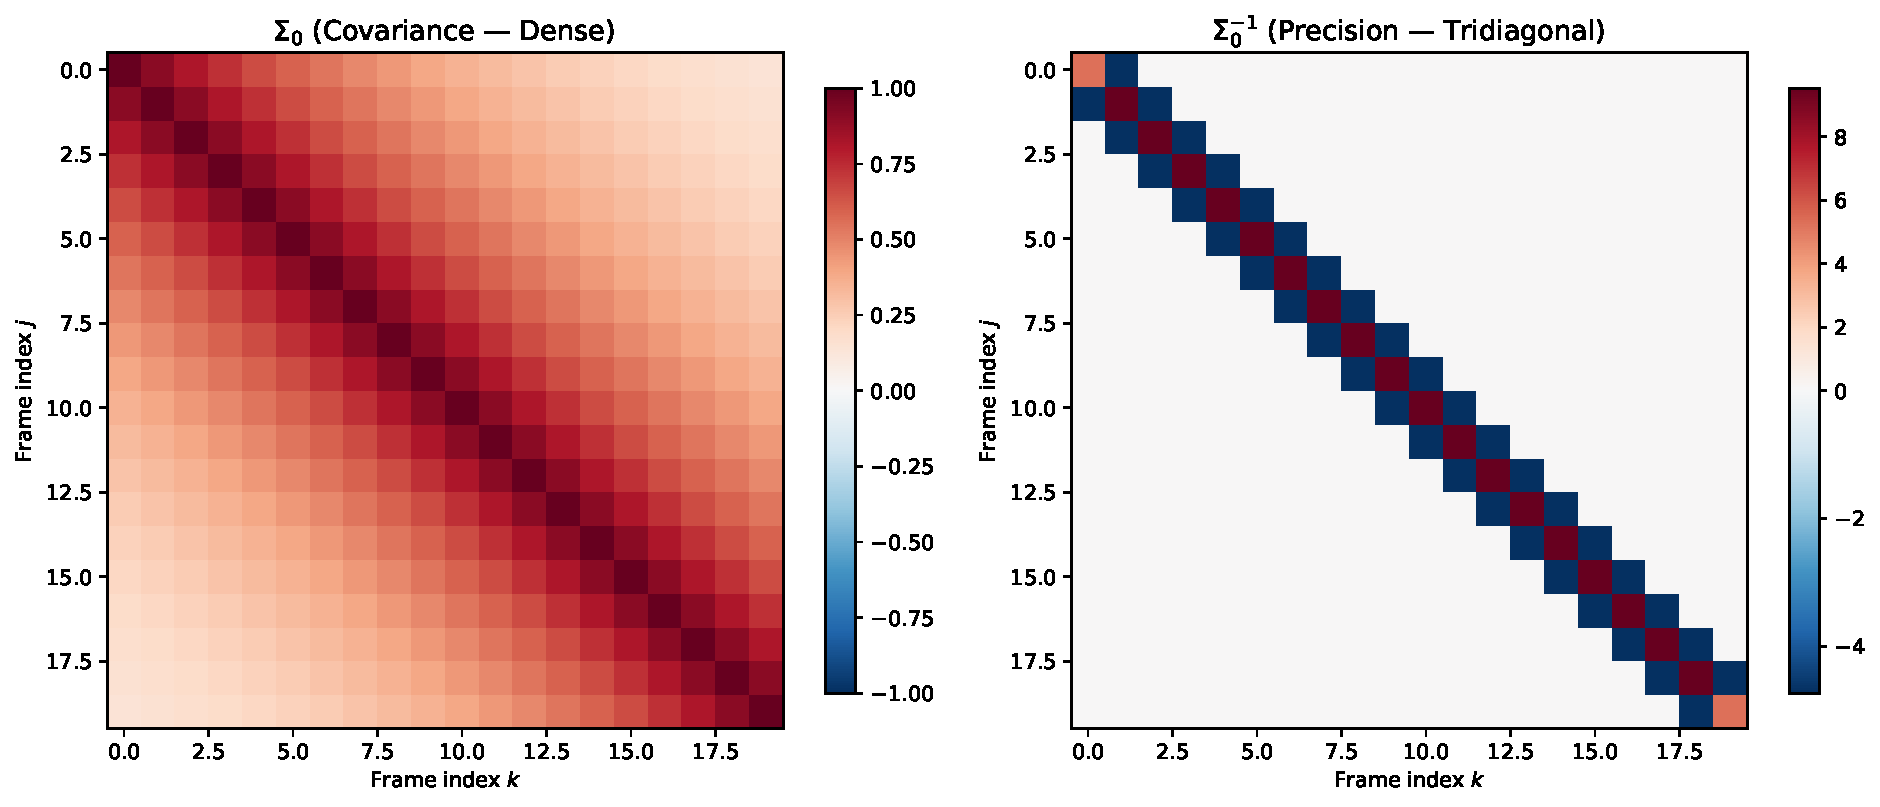
\includegraphics[width=0.95\textwidth]{figures/fig1_sigma0_vs_prec0.pdf}
  \caption{Left: the covariance $\Sigma_0$ is dense, with entries decaying as $\alpha^{|j-k|}$.  Right: the precision $\Sigma_0^{-1}$ is tridiagonal, encoding only nearest-neighbour couplings.  The contrast illustrates the duality between marginal correlations (covariance) and conditional correlations (precision).}
  \label{fig:sigma0}
\end{figure}

\subsection{Explicit $5 \times 5$ matrices at selected diffusion times}

To build intuition, we display the full numerical values for $K = 4$ (5 frames) at four diffusion times.  All entries are rounded to 4 decimal places.

\medskip
\noindent\textbf{At $t = 0$ ($\Dt = 0$, pure signal):}
\begin{equation}\label{eq:numerical-t0}
\Sigma_0^{-1} = \begin{pmatrix}
5.2632 & -4.7368 & 0 & 0 & 0 \\
-4.7368 & 9.5263 & -4.7368 & 0 & 0 \\
0 & -4.7368 & 9.5263 & -4.7368 & 0 \\
0 & 0 & -4.7368 & 9.5263 & -4.7368 \\
0 & 0 & 0 & -4.7368 & 5.2632
\end{pmatrix}.
\end{equation}
Perfectly tridiagonal.  The zero entries encode conditional independence: $a_j \perp a_k \mid \text{rest}$ for $|j-k| \geq 2$.

\medskip
\noindent\textbf{At $t = 0.3$ ($\Dt = 0.4512$):}
\begin{equation}\label{eq:numerical-t03}
\Sigma_t^{-1} = \begin{pmatrix}
1.4691 & -0.4530 & -0.2801 & -0.1823 & -0.1332 \\
-0.4530 & 1.5967 & -0.3831 & -0.2493 & -0.1823 \\
-0.2801 & -0.3831 & 1.6275 & -0.3831 & -0.2801 \\
-0.1823 & -0.2493 & -0.3831 & 1.5967 & -0.4530 \\
-0.1332 & -0.1823 & -0.2801 & -0.4530 & 1.4691
\end{pmatrix}.
\end{equation}
The tridiagonal zeros are now filled, but with entries significantly smaller than the tridiagonal band.  The first off-diagonal ($\approx -0.45$) is still $\sim 2\times$ larger than the second off-diagonal ($\approx -0.25$).

\medskip
\noindent\textbf{At $t = 1.0$ ($\Dt = 0.8647$):}
\begin{equation}\label{eq:numerical-t10}
\Sigma_t^{-1} = \begin{pmatrix}
1.0345 & -0.1014 & -0.0852 & -0.0728 & -0.0636 \\
-0.1014 & 1.0405 & -0.0975 & -0.0833 & -0.0728 \\
-0.0852 & -0.0975 & 1.0424 & -0.0975 & -0.0852 \\
-0.0728 & -0.0833 & -0.0975 & 1.0405 & -0.1014 \\
-0.0636 & -0.0728 & -0.0852 & -0.1014 & 1.0345
\end{pmatrix}.
\end{equation}
Near-diagonal.  All off-diagonal entries are of similar magnitude---the tridiagonal prominence is lost.

\medskip
\noindent\textbf{At $t = 3.0$ ($\Dt = 0.9975$):}
\begin{equation}\label{eq:numerical-t30}
\Sigma_t^{-1} \approx \begin{pmatrix}
1.0000 & -0.0022 & -0.0020 & -0.0018 & -0.0016 \\
-0.0022 & 1.0000 & -0.0022 & -0.0020 & -0.0018 \\
-0.0020 & -0.0022 & 1.0000 & -0.0022 & -0.0020 \\
-0.0018 & -0.0020 & -0.0022 & 1.0000 & -0.0022 \\
-0.0016 & -0.0018 & -0.0020 & -0.0022 & 1.0000
\end{pmatrix}.
\end{equation}
Essentially the identity.  All inter-frame coupling is below $0.3\%$.  The score is $S(\mathbf{x}, t) \approx -\mathbf{x}/\Dt \approx -\mathbf{x}$, each component independent.

\subsection{$\Sigma_t$ and $\Sigma_t^{-1}$ heatmaps for $K = 19$}

\begin{figure}[H]
  \centering
  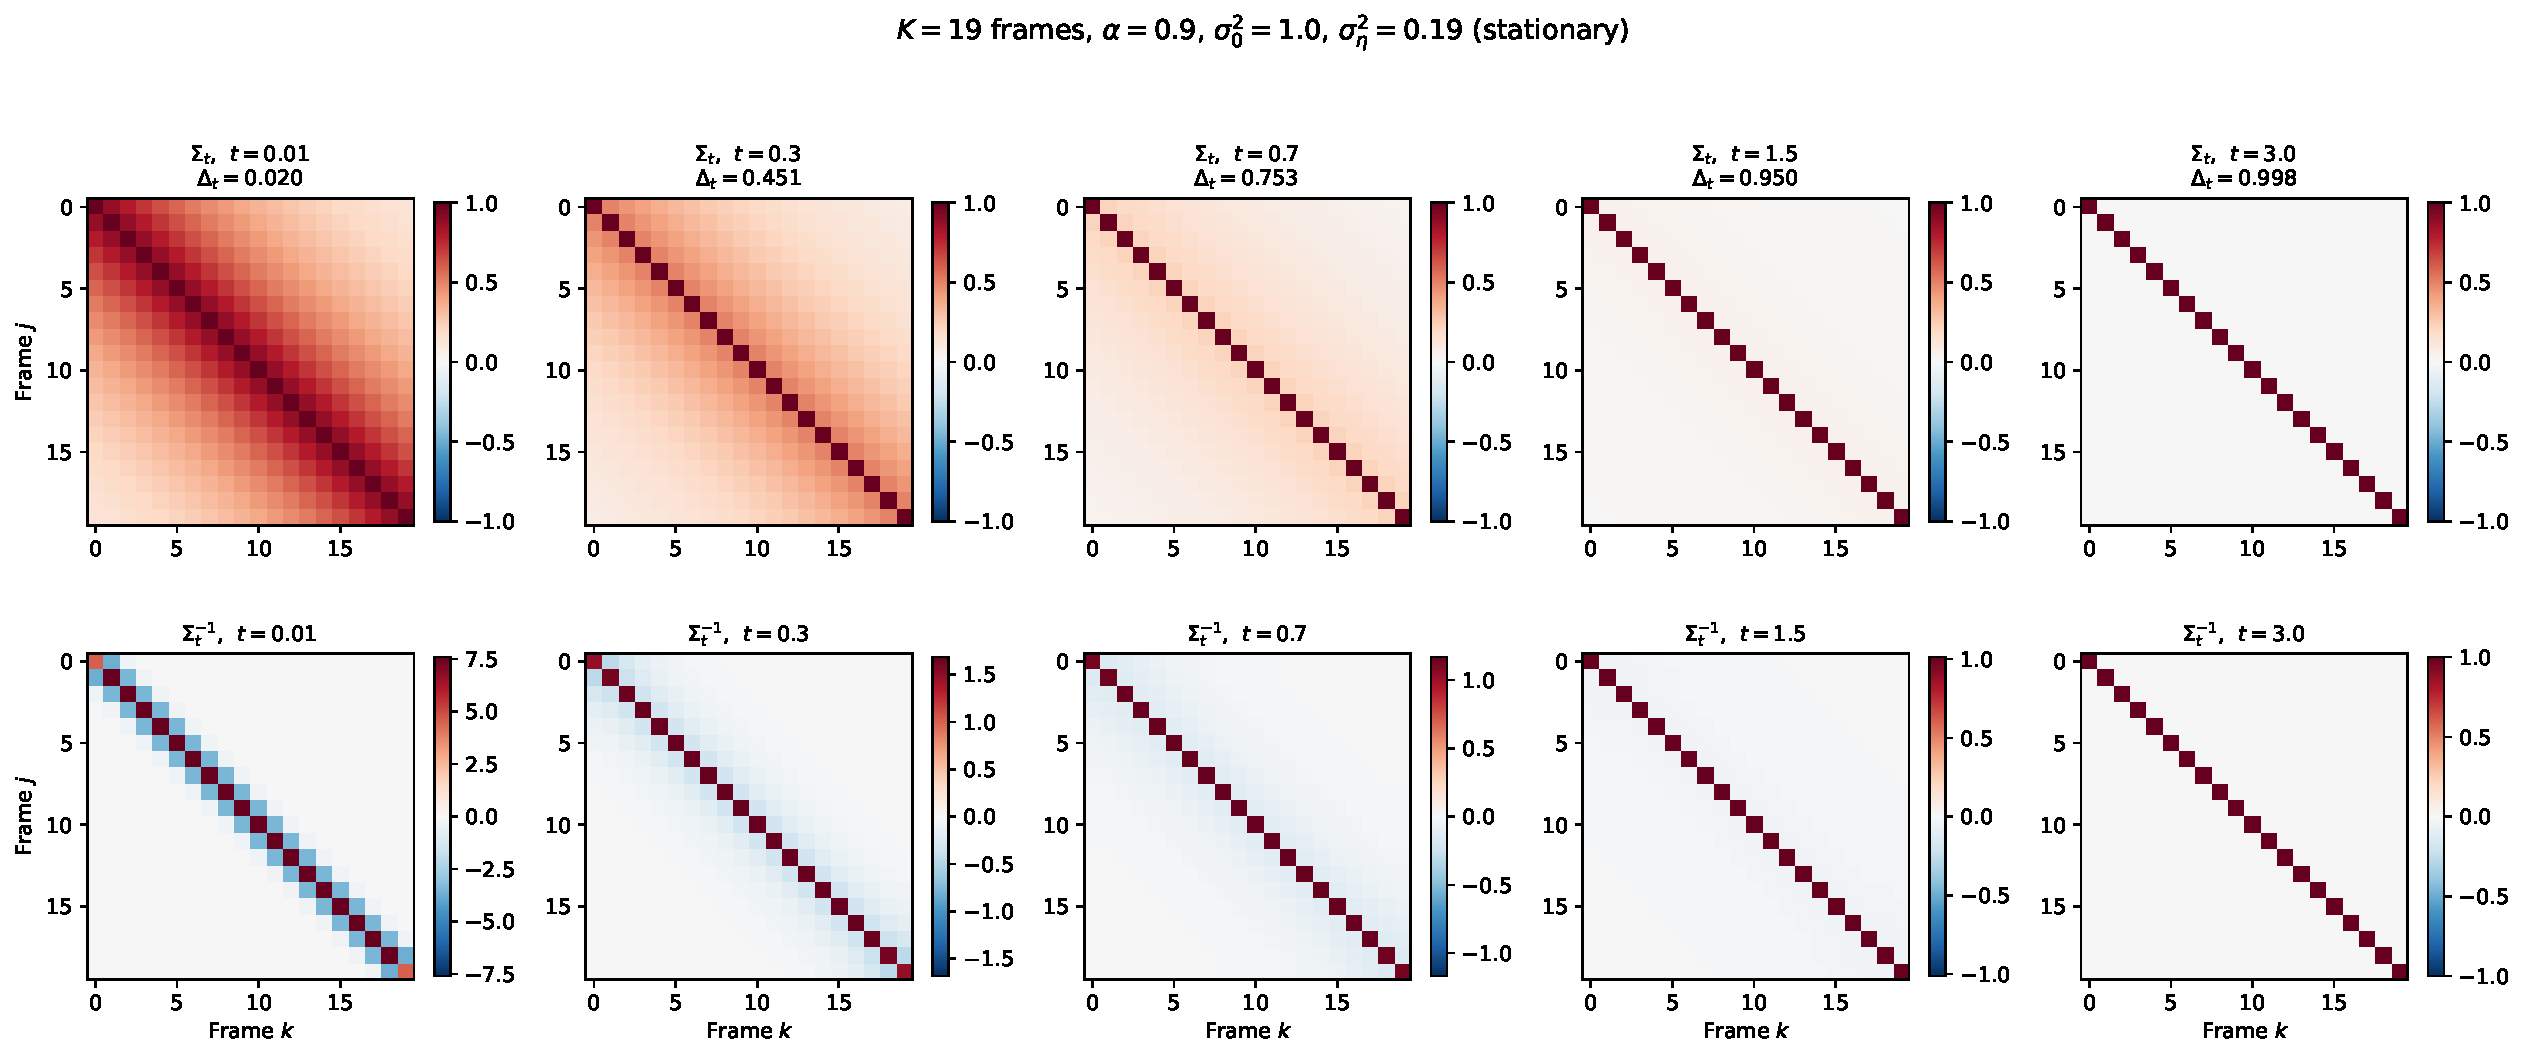
\includegraphics[width=\textwidth]{figures/fig2_sigma_t_panel.pdf}
  \caption{Top row: $\Sigma_t$ at $t = 0.01, 0.3, 0.7, 1.5, 3.0$.  The off-diagonal correlations shrink as $e^{-2t}$.  Bottom row: $\Sigma_t^{-1}$ at the same times.  At $t = 0.01$, the precision is visually tridiagonal.  By $t = 0.3$, the structural zeros are filled but the tridiagonal band remains dominant.  By $t = 3.0$, the matrix is essentially $I$.}
  \label{fig:sigma-t-panel}
\end{figure}

\subsection{How much of $\Sigma_t^{-1}$ lives on the tridiagonal band?}

To quantify the persistence of Markov structure, define the \emph{tridiagonal weight fraction}:
\begin{equation}\label{eq:tridiag-fraction}
  \rho_{\mathrm{tri}}(t) = \frac{\displaystyle\sum_{|j-k| \leq 1} |(\Sigma_t^{-1})_{jk}|}{\displaystyle\sum_{j,k} |(\Sigma_t^{-1})_{jk}|}.
\end{equation}

\begin{figure}[H]
  \centering
  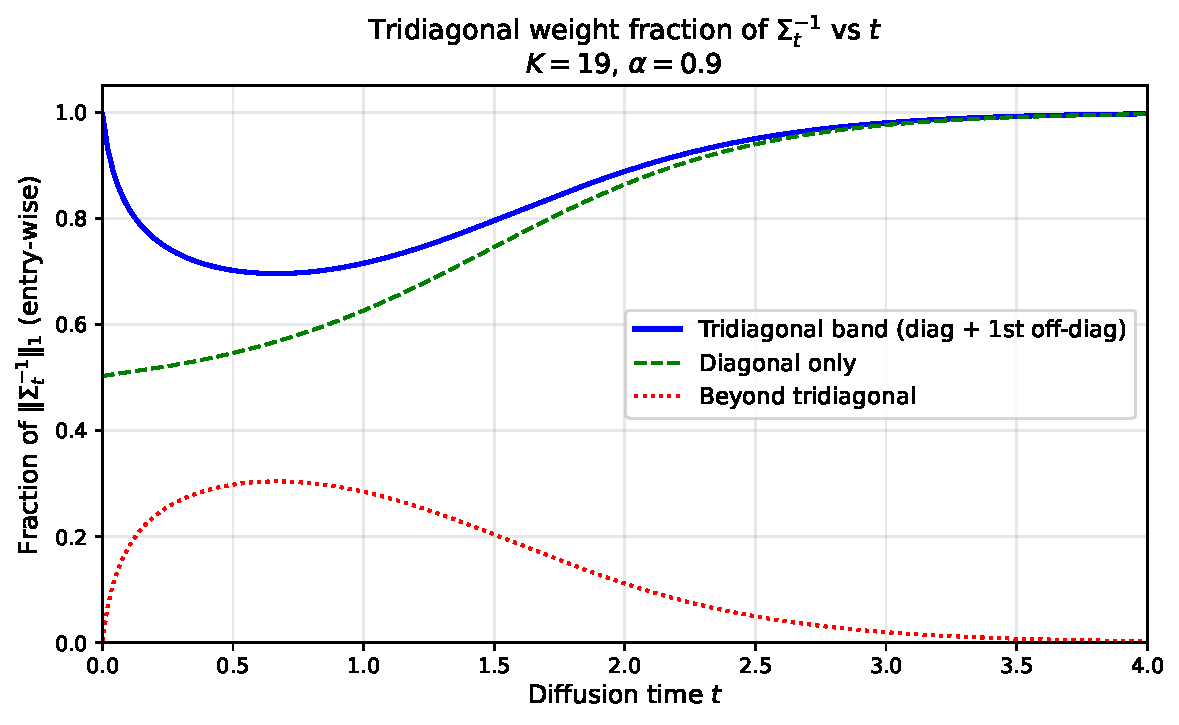
\includegraphics[width=0.7\textwidth]{figures/fig3_tridiag_fraction.pdf}
  \caption{Tridiagonal weight fraction $\rho_{\mathrm{tri}}(t)$ as a function of diffusion time.  At $t = 0$: $\rho_{\mathrm{tri}} = 1$ (perfectly tridiagonal).  The fraction decays monotonically, but the tridiagonal band retains $> 80\%$ of the total weight until $t \approx 0.3$.  At large $t$, the diagonal alone captures nearly all the weight (green dashed), as the matrix approaches $I$.}
  \label{fig:tridiag-fraction}
\end{figure}

\subsection{Row profile: coupling strength as a function of distance}

\begin{figure}[H]
  \centering
  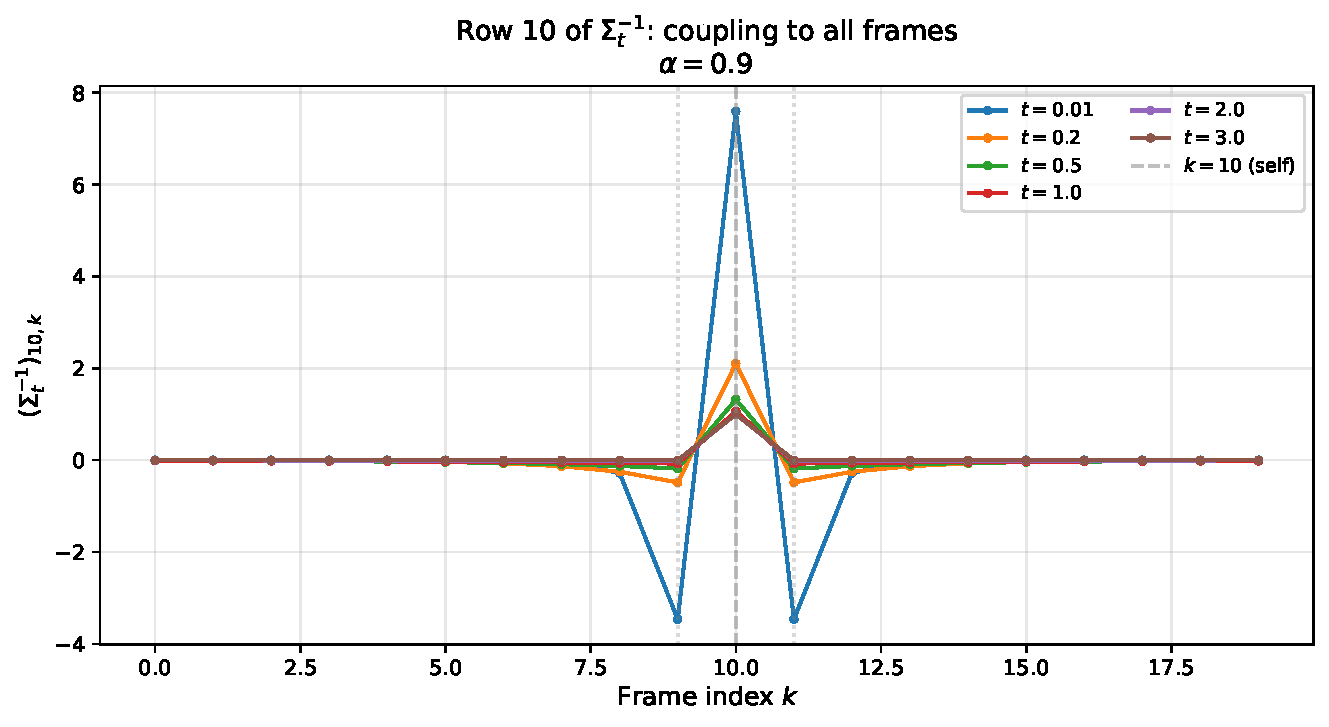
\includegraphics[width=0.7\textwidth]{figures/fig4_row_profile.pdf}
  \caption{Row 10 of $\Sigma_t^{-1}$ (the middle frame's coupling to all other frames) at several diffusion times.  At $t = 0.01$, the coupling is concentrated on the nearest neighbours.  At $t = 0.2$, the coupling has spread to further frames, decaying approximately exponentially with distance.  At large $t$, all couplings vanish.}
  \label{fig:row-profile}
\end{figure}

\subsection{Off-diagonal decay: exponential envelope}

\begin{figure}[H]
  \centering
  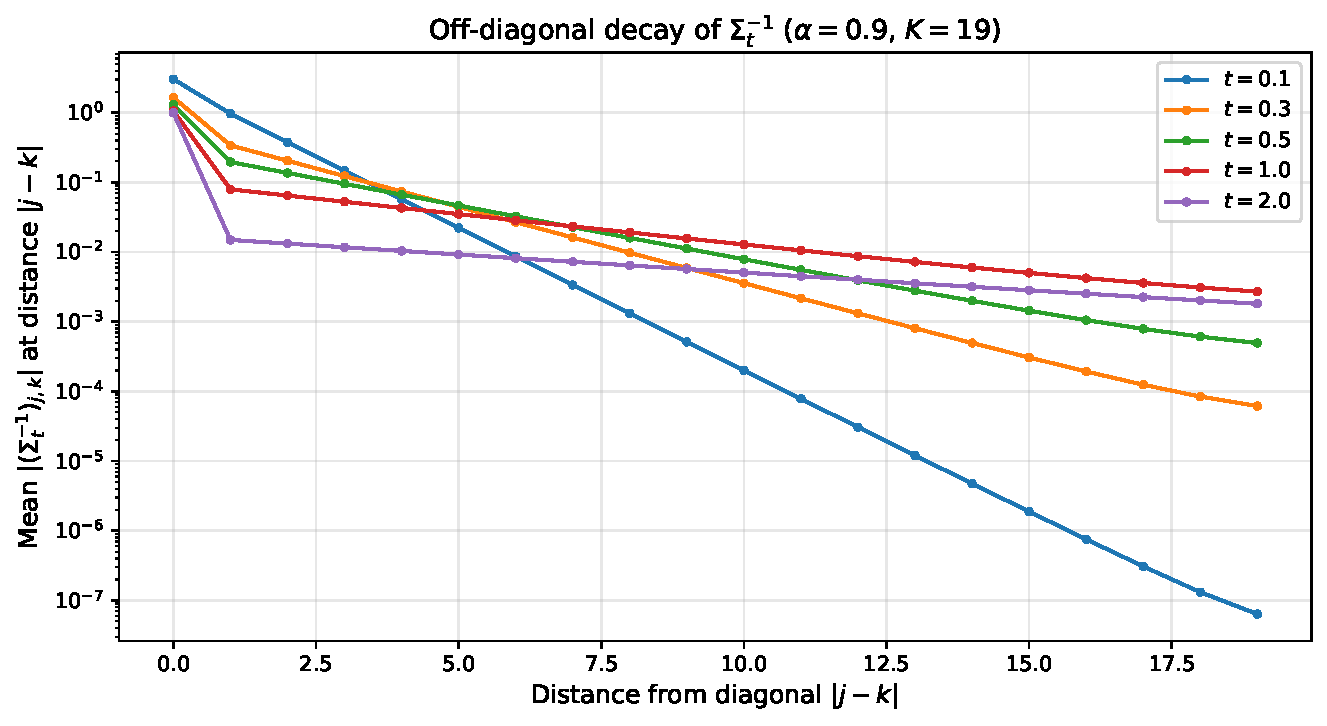
\includegraphics[width=0.7\textwidth]{figures/fig8_offdiag_decay.pdf}
  \caption{Mean absolute value of $(\Sigma_t^{-1})_{jk}$ as a function of the distance $|j-k|$ from the diagonal (log scale).  At all positive $t$, the off-diagonal entries decay approximately exponentially with distance, but the decay rate depends on $t$: slower decay at small $t$ (more long-range coupling).}
  \label{fig:offdiag-decay}
\end{figure}

% ══════════════════════════════════════════════════════════════════════
\section{Eigenvalue Analysis}
\label{sec:eigenvalue-analysis}
% ══════════════════════════════════════════════════════════════════════

\subsection{Spectrum of $\Sigma_0$}

\begin{figure}[H]
  \centering
  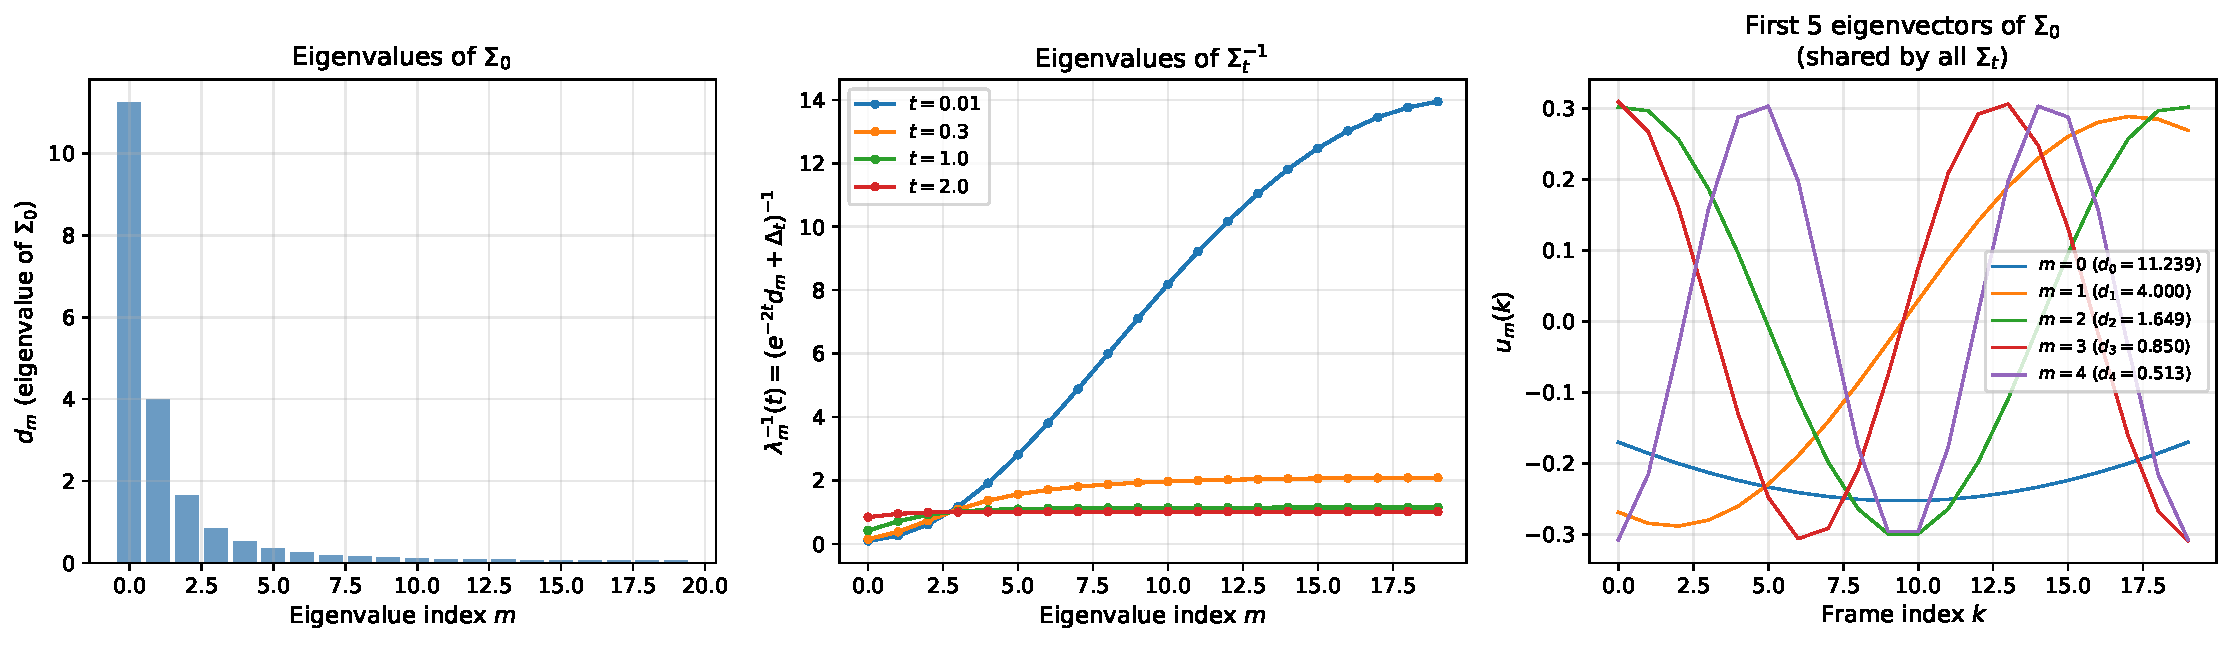
\includegraphics[width=\textwidth]{figures/fig5_eigenvalues.pdf}
  \caption{Left: eigenvalues of $\Sigma_0$, ordered from largest to smallest.  The slow mode ($m = 0$) has $d_0 \approx 10$, while the fast mode ($m = 19$) has $d_{19} \approx 0.028$.  Middle: eigenvalues of $\Sigma_t^{-1}$ at several $t$ values; all converge to 1 as $t \to \infty$.  Right: the first 5 eigenvectors of $\Sigma_0$---smooth, sine-like oscillations, with the $m$-th eigenvector having approximately $m$ zero crossings.}
  \label{fig:eigenvalues}
\end{figure}

\subsection{Eigenvalue trajectories vs.\ diffusion time}

\begin{figure}[H]
  \centering
  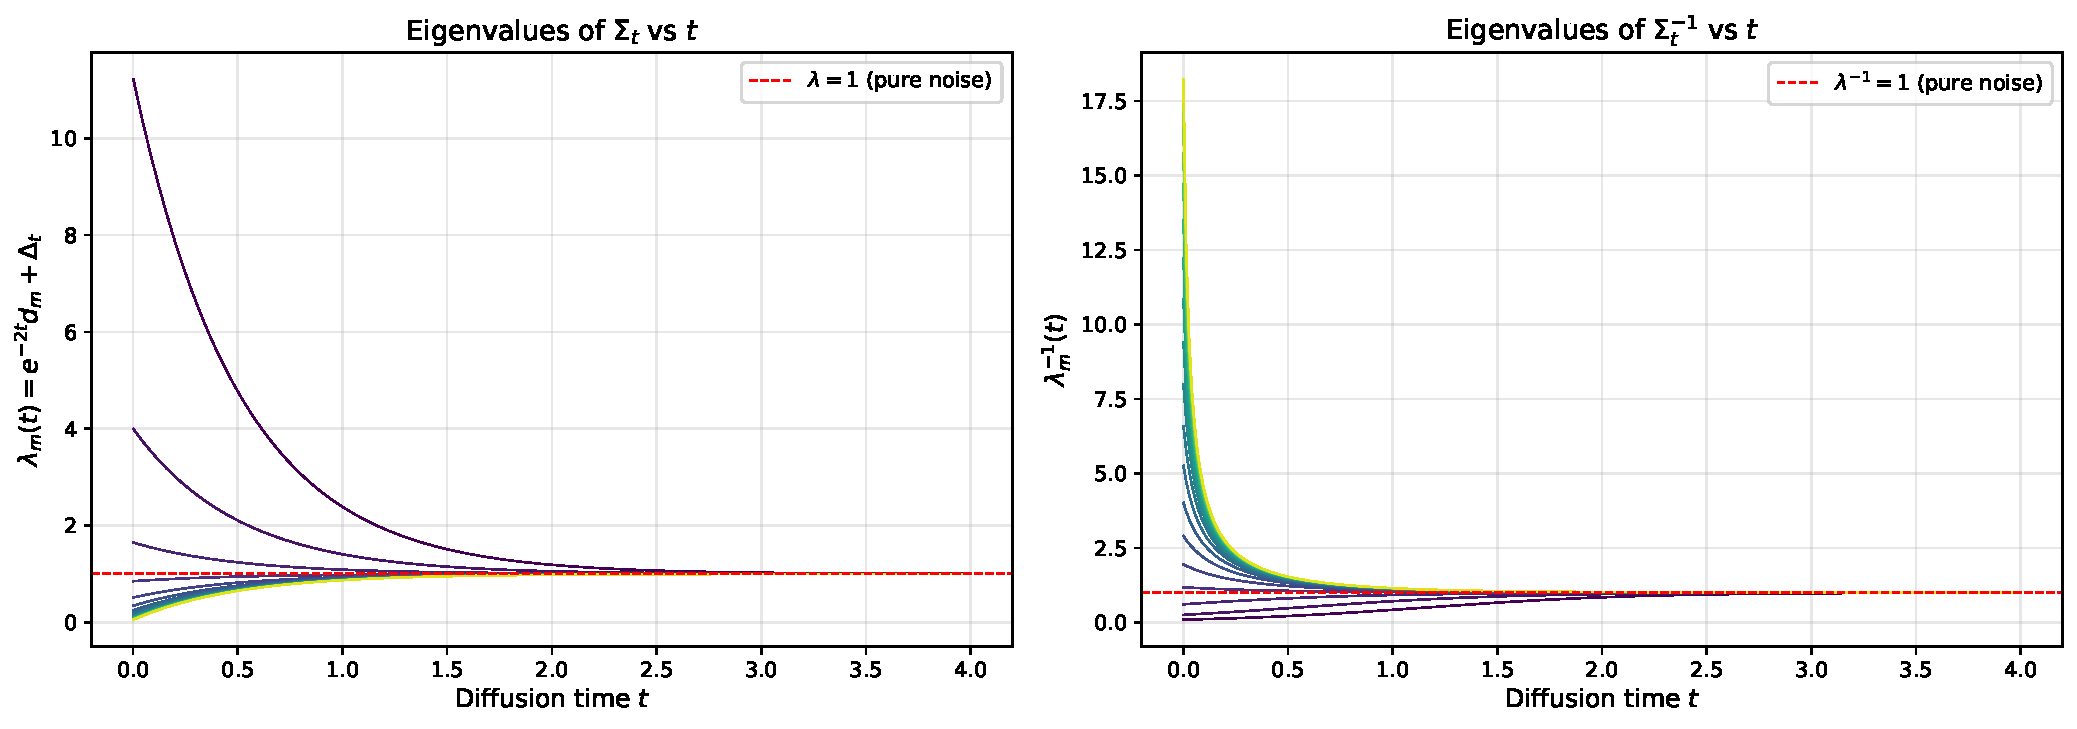
\includegraphics[width=\textwidth]{figures/fig7_eigenvalue_trajectories.pdf}
  \caption{Left: eigenvalues of $\Sigma_t$ as functions of $t$.  Each curve $\lambda_m(t) = e^{-2t}d_m + \Dt$ interpolates from $d_m$ (at $t = 0$) to 1 (as $t \to \infty$).  The slow modes (large $d_m$) approach 1 from above; the fast modes (small $d_m$) approach 1 from below.  Right: the reciprocals $\lambda_m^{-1}(t)$, which are the eigenvalues of $\Sigma_t^{-1}$.  These control the score: large $\lambda_m^{-1}(t)$ means the $m$-th mode contributes strongly to the score.}
  \label{fig:eigenvalue-trajectories}
\end{figure}

\subsection{$\Sigma_t^{-1}$ in the eigenbasis: perfect diagonality}

\begin{figure}[H]
  \centering
  
\includegraphics[width=\textwidth]{figures/fig6_eigenbasis.pdf}
  \caption{The matrix $|U^\top \Sigma_t^{-1} U|$ at four diffusion times.  It is \emph{exactly} diagonal at all $t$, confirming that the eigenvectors of $\Sigma_0$ diagonalise $\Sigma_t^{-1}$ for all $t$ simultaneously.  The diagonal entries are $1/(e^{-2t}d_m + \Dt)$.}
  \label{fig:eigenbasis}
\end{figure}

\subsection{Condition number}

\begin{figure}[H]
  \centering
  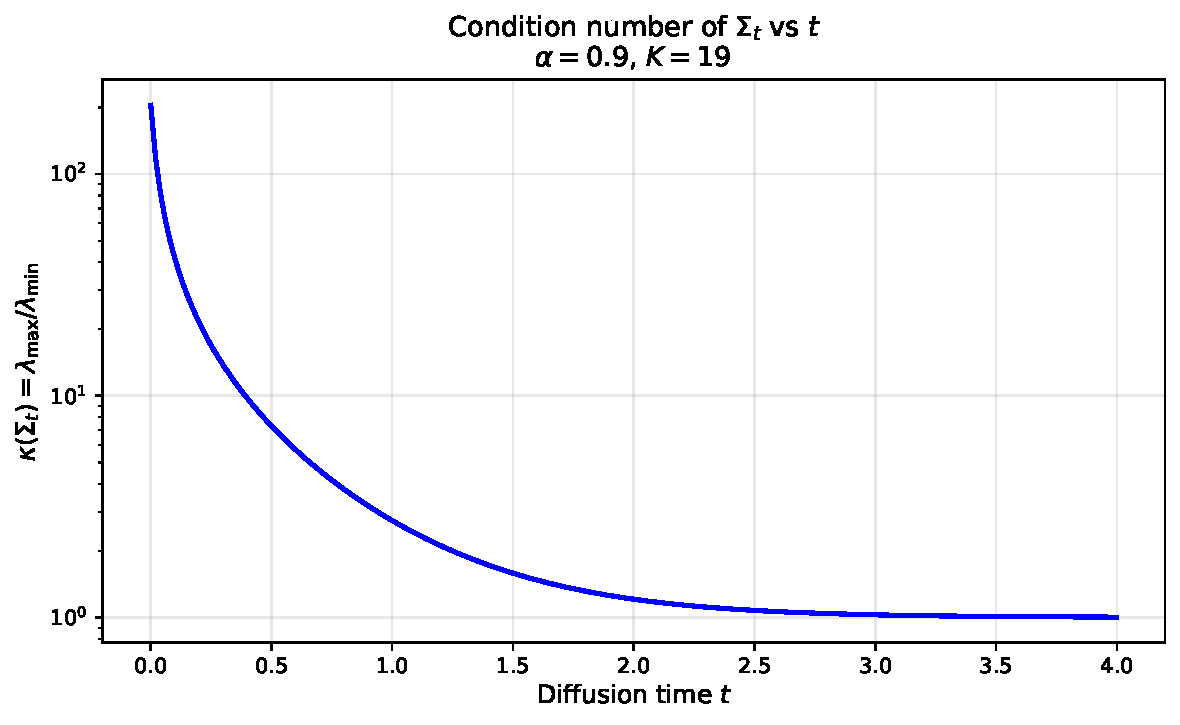
\includegraphics[width=0.65\textwidth]{figures/fig9_condition_number.pdf}
  \caption{Condition number $\kappa(\Sigma_t) = \lambda_{\max}(t)/\lambda_{\min}(t)$ as a function of $t$.  At $t = 0$, $\kappa = d_0/d_K \approx 361$ (highly anisotropic).  As $t \to \infty$, $\kappa \to 1$ (isotropic).  The condition number quantifies how ``stretched'' the Gaussian ellipsoid is: large $\kappa$ means the score is very sensitive to perturbations along the fast-mode directions.}
  \label{fig:condition-number}
\end{figure}

% ══════════════════════════════════════════════════════════════════════
\section{Sensitivity to $\alpha$}
\label{sec:alpha-sensitivity}
% ══════════════════════════════════════════════════════════════════════

The AR(1) parameter $\alpha$ controls the strength of inter-frame correlation.  We examine how $\Sigma_t$ and $\Sigma_t^{-1}$ change as $\alpha$ varies.

\begin{figure}[H]
  \centering
  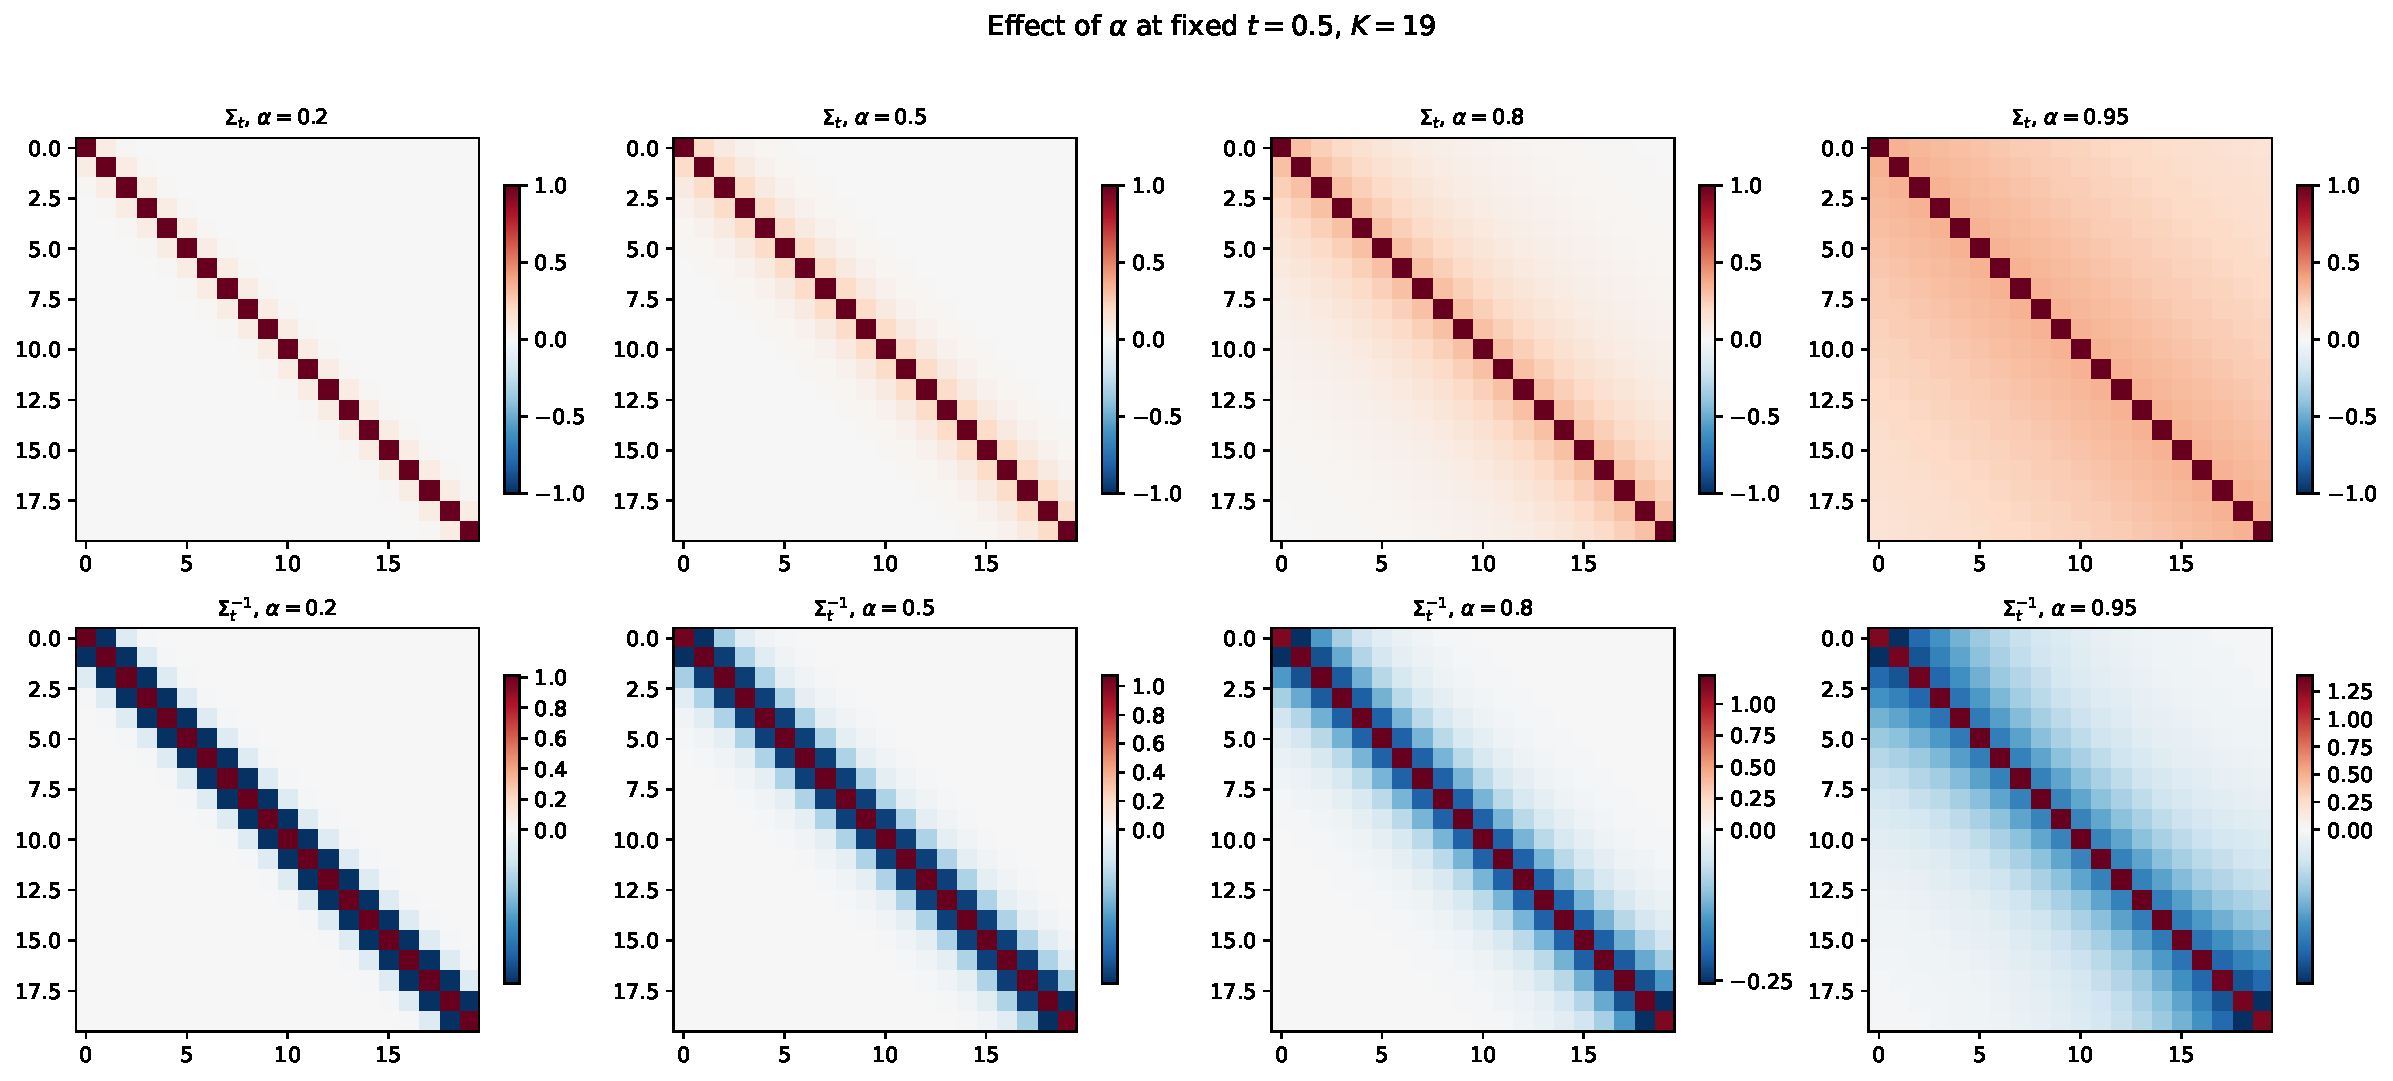
\includegraphics[width=\textwidth]{figures/fig11_alpha_sensitivity.pdf}
  \caption{$\Sigma_t$ (top) and $\Sigma_t^{-1}$ (bottom) at fixed $t = 0.5$ for $\alpha \in \{0.2, 0.5, 0.8, 0.95\}$.  For small $\alpha$, the clean covariance is already nearly diagonal, so diffusion noise has little structural effect.  For large $\alpha$, the clean covariance is highly correlated, and the precision at $t = 0.5$ retains significant off-tridiagonal weight---the Markov structure is more persistent in the score for strongly correlated sequences.}
  \label{fig:alpha-sensitivity}
\end{figure}

\begin{observation}[$\alpha$ controls the ``lifetime'' of Markov structure in the score]\label{obs:alpha-lifetime}
For large $\alpha$, the eigenvalue spread $d_{\max}/d_{\min} \sim (1+\alpha)^2/(1-\alpha)^2$ is large.  The slow mode has half-life $t_0^* \approx \frac{1}{2}\ln d_0$, which grows as $\alpha \to 1$.  Therefore, for strongly correlated AR(1) chains, the score retains inter-frame coupling to larger diffusion times.

Conversely, for small $\alpha$ (weakly correlated), the eigenvalues cluster near $\siginf \approx 1$, the condition number is small, and the Markov structure in the score is washed out quickly.
\end{observation}

% ══════════════════════════════════════════════════════════════════════
\section{Component-Wise Score Structure}
\label{sec:score-structure}
% ══════════════════════════════════════════════════════════════════════

Combining the algebraic and numerical results, we can now give a complete picture of the $k$-th component of the joint score.

\subsection{In the original frame basis}

From Corollary 5.1 of the previous note:
\begin{equation}\label{eq:sk-original}
  S_k(\mathbf{x}, t) = -\sum_{j=0}^{K} (\Sigma_t^{-1})_{kj}\,(x_j - \mu_{t,j}).
\end{equation}
At $t = 0$, $\Sigma_t^{-1} = \Sigma_0^{-1}$ is tridiagonal, so:
\begin{equation}\label{eq:sk-clean}
  S_k(\mathbf{x}, 0) = -(\Sigma_0^{-1})_{k,k-1}(x_{k-1} - \mu_{a,k-1}) - (\Sigma_0^{-1})_{k,k}(x_k - \mu_{a,k}) - (\Sigma_0^{-1})_{k,k+1}(x_{k+1} - \mu_{a,k+1}).
\end{equation}
This is a \textbf{nearest-neighbour coupling}: the score at frame $k$ depends only on frames $k-1, k, k+1$.  This is the Markov structure manifesting in the score.

For $t > 0$, $\Sigma_t^{-1}$ is dense, and $S_k$ couples to \emph{all} frames.  However, the coupling strength $|(\Sigma_t^{-1})_{kj}|$ decays with distance $|k - j|$ (approximately exponentially, as shown in Figure~\ref{fig:offdiag-decay}).

\subsection{In the eigenbasis}

From Theorem~\ref{thm:decoupling}:
\begin{equation}\label{eq:score-eigenbasis}
  \tilde{S}_m(\tilde{\mathbf{x}}, t) = -\frac{\tilde{x}_m - \tilde{\mu}_{t,m}}{e^{-2t}d_m + \Dt}.
\end{equation}
Each mode is an independent scalar denoiser.  The ``effective SNR'' of the $m$-th mode is:
\begin{equation}\label{eq:effective-snr}
  \text{SNR}_m(t) = \frac{e^{-2t}\,d_m}{\Dt}.
\end{equation}
When $\text{SNR}_m(t) \gg 1$, the $m$-th mode still carries useful signal and the score is informative.  When $\text{SNR}_m(t) \ll 1$, the mode is dominated by noise and the score simply pushes $\tilde{x}_m$ toward the mean.

\subsection{Connecting the two bases: the score in frame space from the spectral decomposition}

Using \eqref{eq:spectral-sum}:
\begin{equation}\label{eq:sk-spectral}
  S_k(\mathbf{x}, t) = -\sum_{m=0}^{K}\;\frac{1}{e^{-2t}d_m + \Dt}\;\sum_{j=0}^{K} u_m(k)\,u_m(j)\,(x_j - \mu_{t,j}).
\end{equation}
This decomposes the coupling $(\Sigma_t^{-1})_{kj}$ into spectral contributions:
\begin{equation}\label{eq:precision-spectral}
  (\Sigma_t^{-1})_{kj} = \sum_{m=0}^{K} \frac{u_m(k)\,u_m(j)}{e^{-2t}d_m + \Dt}.
\end{equation}
The entry $(\Sigma_t^{-1})_{kj}$ is a weighted sum of products $u_m(k)\,u_m(j)$ over all modes.  For the tridiagonal Markov case, the eigenvectors $u_m(k)$ are spatially localised (sine-like), and nearby frames share similar eigenvector values.  This is why $|(\Sigma_t^{-1})_{kj}|$ decays with distance $|k - j|$ even for $t > 0$.


% ══════════════════════════════════════════════════════════════════════
\section{Why the Inverse of a Tridiagonal Matrix Is Full}
\label{sec:tridiag-inverse}
% ══════════════════════════════════════════════════════════════════════

This section explains the algebraic mechanism behind the filling of zeros in $\Sigma_t^{-1}$, a point raised by M\'ezard during the meeting.

\begin{proposition}[Inverse of a tridiagonal matrix is full]\label{prop:tridiag-full}
Let $T$ be an $n \times n$ symmetric, positive definite, tridiagonal matrix with non-zero off-diagonal entries.  Then $(T^{-1})_{jk} \neq 0$ for all $j, k$.
\end{proposition}

\begin{proof}[Proof sketch]
Write $T = LDL^\top$ (Cholesky or $LDL^\top$ decomposition).  Since $T$ is tridiagonal, $L$ is lower bidiagonal: $L_{ij} \neq 0$ only for $j = i$ or $j = i-1$.  The inverse $T^{-1} = L^{-\top}D^{-1}L^{-1}$.  The inverse of a bidiagonal matrix is \emph{full} (lower/upper triangular with all entries non-zero), and the product of two full triangular matrices is full.
\end{proof}

\begin{remark}[Connection to Fourier modes]\label{rem:fourier}
As M\'ezard noted, one can understand this in Fourier space.  The tridiagonal matrix $T$ has eigenvalues $\lambda_m = a + 2b\cos\theta_m$ (approximately), which are all distinct.  The inverse has eigenvalues $1/\lambda_m$, but the \emph{eigenvectors} are shared.  Expressing $T^{-1}$ as a sum over eigenvector outer products $\sum_m (1/\lambda_m)\,\mathbf{u}_m \mathbf{u}_m^\top$, every entry receives a contribution from every mode (since $u_m(k) \neq 0$ for all $k, m$ in general).  No cancellation makes $(T^{-1})_{jk}$ exactly zero.
\end{remark}

Now, $\Sigma_t^{-1}$ involves the inverse of $B = e^{-2t}I + \Dt\,\Sigma_0^{-1}$, which is tridiagonal (a diagonal shift of a tridiagonal matrix is still tridiagonal).  By Proposition~\ref{prop:tridiag-full}, $B^{-1}$ is full, and the product $\Sigma_0^{-1} \cdot B^{-1}$ is full.  This is the precise mechanism by which the diffusion noise destroys the tridiagonal sparsity pattern.


% ══════════════════════════════════════════════════════════════════════
\section{Summary of Key Results}
\label{sec:summary}
% ══════════════════════════════════════════════════════════════════════

\begin{keyresult}[Main findings]
\begin{enumerate}[label=\textbf{\arabic*.}, leftmargin=2em]
  \item \textbf{Four representations of $\Sigma_t^{-1}$:}
  \begin{align}
    \Sigma_t^{-1} &= \tfrac{1}{\Dt}\,(I + \gamma_t\Sigma_0)^{-1} & & \text{(Factored)} \label{eq:rep1}\\
    &= \Sigma_0^{-1}\,(e^{-2t}I + \Dt\Sigma_0^{-1})^{-1} & & \text{(M\'ezard)} \label{eq:rep2}\\
    &= \tfrac{1}{\Dt}I - \tfrac{e^{-2t}}{\Dt^2}\Sigma_0(\Sigma_0^{-1} + \tfrac{e^{-2t}}{\Dt}I)^{-1} & & \text{(Woodbury)} \label{eq:rep3}\\
    &= U\,\diag\!\bigl(1/(e^{-2t}d_m + \Dt)\bigr)\,U^\top & & \text{(Spectral)} \label{eq:rep4}
  \end{align}

  \item \textbf{At $t = 0$: Markov structure.}  $\Sigma_0^{-1}$ is tridiagonal---nearest-neighbour coupling only.

  \item \textbf{At $t > 0$: zeros fill in.}  The inversion in M\'ezard's form \eqref{eq:rep2} maps the tridiagonal structure to a full matrix.  The beyond-tridiagonal entries decay approximately exponentially with frame distance and with $e^{-2t}$.

  \item \textbf{Tridiagonal weight fraction $\rho_{\mathrm{tri}}(t)$} decays monotonically from 1 (at $t = 0$) toward $1/(K+1)$ (at $t \to \infty$, uniform over all entries of $I$).  The Markov ``fingerprint'' persists most strongly at small $t$ and for large $\alpha$.

  \item \textbf{Shared eigenvectors.}  $\Sigma_t$, $\Sigma_t^{-1}$, and $\Sigma_0$ all share the same eigenvectors $U$, for all $t$.  Only the eigenvalues change: $\lambda_m(t) = e^{-2t}d_m + \Dt$.

  \item \textbf{Full decoupling in the eigenbasis.}  The rotated score $\tilde{S}_m = -(\tilde{x}_m - \tilde{\mu}_{t,m})/(e^{-2t}d_m + \Dt)$ is independent across modes.  The reverse SDE splits into $K+1$ independent scalar processes.

  \item \textbf{This decoupling is Gaussian, not Markov.}  Any Gaussian $P_0$ (with any covariance structure) admits an eigenbasis in which $\Sigma_t^{-1}$ is diagonal.  The Markov property determines the specific form of the eigenvectors (sine-like, spatially localised) and eigenvalues (the formula \eqref{eq:eigvals-cov0}), but does not by itself enable the decoupling.
\end{enumerate}
\end{keyresult}


% ══════════════════════════════════════════════════════════════════════
\section{Discussion and Next Steps}
\label{sec:discussion}
% ══════════════════════════════════════════════════════════════════════

\subsection{What Markovianity contributes (and what it does not)}

The analysis reveals a precise decomposition of roles:

\medskip
\begin{tabular}{@{}lp{10cm}@{}}
\toprule
\textbf{Property} & \textbf{Source} \\
\midrule
$\Sigma_0^{-1}$ is tridiagonal & Markov property of $P_0(\mathbf{a})$ \\
$\Sigma_t$ and $\Sigma_t^{-1}$ share eigenvectors with $\Sigma_0$ & Gaussianity of $P_0(\mathbf{a})$ + i.i.d.\ OU noise \\
Score decouples in eigenbasis & Gaussianity of $P_0(\mathbf{a})$ \\
Eigenvectors are sine-like / spatially localised & Tridiagonal (Markov) structure of $\Sigma_0^{-1}$ \\
Eigenvalue spectrum has specific form \eqref{eq:eigvals-cov0} & AR(1) dynamics (value of $\alpha$, $\sigeta$) \\
Off-diagonal entries of $\Sigma_t^{-1}$ decay with distance & Eigenvector localisation (indirect Markov effect) \\
\bottomrule
\end{tabular}

\medskip
The key takeaway: Markovianity provides the \emph{specific structural form} of the eigenvectors and eigenvalues, but the \emph{existence} of a fully decoupled basis is a generic Gaussian phenomenon.

\subsection{Next steps}

Following M\'ezard's roadmap from the meeting:
\begin{enumerate}[label=(\roman*), nosep]
  \item \textbf{Enrich $P_0(\mathbf{a})$}: give $P_0$ its own non-trivial covariance structure within each frame (multivariate frames), to disentangle the effect of intra-frame correlations from the Markov inter-frame structure.
  \item \textbf{Mixture of Gaussians}: replace the Gaussian $P_0$ with a mixture.  The score becomes nonlinear in $\mathbf{x}$, and the eigenbasis decoupling breaks.  The question is: does the Markov structure of the score (nearest-neighbour dominance) survive in the non-Gaussian case?
  \item \textbf{Quantify the ``Markov residual'' in the score}: define indicators that measure how close $\Sigma_t^{-1}$ is to tridiagonal as a function of $t$, beyond the simple weight fraction $\rho_{\mathrm{tri}}(t)$ used here.
  \item \textbf{Connect to the Kalman smoother}: the backward pass of the Kalman smoother is the propagator that computes the posterior mean $\langle a_k \rangle_{\mathbf{a}|\mathbf{x}}$ in $O(K)$ time.  Understand how the smoother gain relates to the spectral decomposition.
\end{enumerate}

% ══════════════════════════════════════════════════════════════════════
\section{Notation Reference}
\label{sec:notation}
% ══════════════════════════════════════════════════════════════════════

\begin{center}
\small
\begin{tabular}{@{}ll@{}}
\toprule
\textbf{Symbol} & \textbf{Meaning} \\
\midrule
$K$ & Number of AR(1) steps; $K+1$ frames total (indices $0, \dots, K$) \\
$t \geq 0$ & Diffusion (OU noise) time \\
$\alpha \in (-1, 1)$ & AR(1) contraction coefficient \\
$\sigzero$ & Variance of initial frame $a_0$ \\
$\sigeta$ & AR(1) innovation variance \\
$\siginf = \sigeta/(1-\alpha^2)$ & Stationary variance \\
$\Dt = 1 - e^{-2t}$ & OU noise variance at diffusion time $t$ \\
$\gamma_t = e^{-2t}/\Dt$ & Signal-to-noise ratio \\
$\Sigma_0$ & $(K\!+\!1) \times (K\!+\!1)$ clean covariance; $(\Sigma_0)_{jk} = \siginf\alpha^{|j-k|}$ (stationary) \\
$\Sigma_t = e^{-2t}\Sigma_0 + \Dt I$ & Noisy covariance \\
$\bm{\mu}_a, \bm{\mu}_t = e^{-t}\bm{\mu}_a$ & Clean / noisy mean \\
$d_m$ & $m$-th eigenvalue of $\Sigma_0$ ($d_0 \geq d_1 \geq \cdots \geq d_K$) \\
$\mathbf{u}_m$ & $m$-th eigenvector of $\Sigma_0$ (shared by $\Sigma_t$ and $\Sigma_t^{-1}$ for all $t$) \\
$U = [\mathbf{u}_0 | \cdots | \mathbf{u}_K]$ & Orthogonal eigenvector matrix \\
$\lambda_m(t) = e^{-2t}d_m + \Dt$ & $m$-th eigenvalue of $\Sigma_t$ \\
$\tilde{\mathbf{x}} = U^\top\mathbf{x}$ & Noisy trajectory in the eigenbasis \\
$S(\mathbf{x}, t) = -\Sigma_t^{-1}(\mathbf{x} - \bm{\mu}_t)$ & Joint score \\
$\tilde{S}_m = -(\tilde{x}_m - \tilde{\mu}_{t,m})/\lambda_m(t)$ & Score in the eigenbasis (independent per mode) \\
$\rho_{\mathrm{tri}}(t)$ & Tridiagonal weight fraction of $\Sigma_t^{-1}$ \\
\bottomrule
\end{tabular}
\end{center}

\end{document}
